\section{서론}

\subsection{연구의 필요성}

천체를 관측할 때 초점을 맞춘다면 관측할 천체의 모습이 더 선명하게 보인다. 일반적으로 대부분 망원경은 초점을 손으로 맞출 수 있게 설계되어있다. 천체망원경으로 사진 관측을 할 때 정확한 초점 조절은 사진의 품질에 영향을 미치는 요소 중의 하나이다. 초점 조정 시 어려운 점은 초점을 조정하기 위해 초점 조절 노브에 손이 닿으면 진동이 발생하고, 그 진동이 사진의 품질에 영향을 준다. 또한, 초점을 조절할 때 손으로 돌리는 것은 미세한 조정에는 어려움이 있다. 또한, 초점이 완벽하게 맞지 않았는데도 이러한 사진을 찍기 위해서 초점을 맞추는데 많은 시간을 투자해야 한다. 이렇듯 사진을 통하여 정밀한 천체의 사진이 필요한 경우 사람의 손으로는 무리가 있다. 하지만 모터 초점 조절 장치가 있다면 손으로 초점을 맞추는 것보다 정확하게 초점을 맞출 수 있게 된다. 

The present invention provides a temperature compensating focuser and method for use with a telescope having a focus which changes with ambient temperature. \cite{persha2001temperature}
\begin{figure}[h]
	\begin{subfigure}{0.5\textwidth}
		
\includegraphics[width=0.9\linewidth, height=5cm]{before} 
		\caption{초점 맞추기 전}
		\label{fig:before}
	\end{subfigure}
	\begin{subfigure}{0.5\textwidth}
		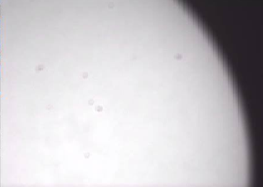
\includegraphics[width=0.9\linewidth, height=5cm]{after}
		\caption{초점 맞춘 후}
		\label{fig:after}
	\end{subfigure}
	\caption{초점을 맞추기 전과 후 비교}
	\label{fig:image1}
\end{figure}
Fig.1.(a), Fig.1.(b)에서 알 수 있듯이 모터 초점 조절 장치를 이용하여 초점을 맞추면 아무것도 하지 않고 그냥 관측했을 때에 비해서 훨씬 정확하게 천체를 관측할 수 있게 된다. Fig.1.(a)와 Fig.1.(b)를 비교하여 보면 Fig.1.(b)의 표면이 훨씬 더 선명하다는 사실을 알 수 있다. 하지만, 모터를 이용하여 초점을 맞춘다고 해도 우리 눈으로 초점을 맞추는 것이기 때문에 정확하지 않을 수 있다. 이러한 문제를 해결하기 위하여 만들어진 자동 초점 조절 장치가 있다. 자동 초점 조절 장치가 현재 개발된 제품이 미국 Starizona 회사의 Micro Touch이다. 이 제품은 자동 초점 조절 시스템이 구현이 잘 되어 있으나, 가격이 499달러로 부담 이 있을 수 있다. 또한, 실제로 모터 초점 조절 장치와 연계해 초점을 맞춰주는 다른 Software도 몇 종류가 있으나 오류가 발생하는 경우가 있다. 따라서 천체망원경의 모터 초점 조절 장치의 컨트롤러 구동 시스템을 개발하면 여러 천체를 관측하는 데 있어서 보다 정확한 사진들을 얻을 수 있을 것이다.

%\begin{wrapfigure}{l}{0.3\textwidth}
%	
\includegraphics[width=1\linewidth]{before}
%	\caption{초점 맞추기 전}
%	\label{fig:before}
%\end{wrapfigure}

\subsection{연구목적}

본 논문에서 제안된 방법은 사람이 손으로 제어하는 것보다 정밀하고 빠르게 천체망원경의 초점을 맞출 수 있도록 편의성을 제공하기 위한 기반을 제공하기 위함이다. 이 연구는 Arduino를 이용하여 천체망원경을 이용한 천체관측을 시행할 때 필요한 모터 초점 조절 장치를 조정할 수 있는 모터 초점 조절 장치 컨트롤러 구동 시스템을 구현하고, 초점을 조정하는 알고리즘을 만들어서 천체의 초점을 맞출 수 있도록 한다. 그리고 이와 통신을 할 수 있는 시스템도 개발하여 편의성을 늘리고, ASCOM 드라이버를 제작하여 컴퓨터와의 통신을 가능하게 하는 것이 이 연구의 목표이다.